\documentclass[conference]{IEEEtran}
\IEEEoverridecommandlockouts
% The preceding line is only needed to identify funding in the first footnote. If that is unneeded, please comment it out.
\usepackage{cite}
\usepackage{amsmath,amssymb,amsfonts}
\usepackage{algorithmic}
\usepackage{graphicx}
\usepackage{textcomp}
\usepackage{xcolor}
\def\BibTeX{{\rm B\kern-.05em{\sc i\kern-.025em b}\kern-.08em
    T\kern-.1667em\lower.7ex\hbox{E}\kern-.125emX}}
\begin{document}

\title{Agricultural Resources Rental App\\
{\footnotesize \textsuperscript{}}
}

\author{\IEEEauthorblockN{Sagar Nakum}
\IEEEauthorblockA{
\textit 201701182@daiict.ac.in\\
\textit Dhirubhai Ambani Institute of Information and Communication Technology \\
\textit Gandhinagar, India \\
Mentor : Prof.JayPrakash Lalchandani }
}

\maketitle

\begin{abstract}
 India has the second-highest population in the world and around 70 per cent of the population of our country is heavily dependent on agriculture and we earn 65 per cent of money through agriculture.\\
 But when it comes to technology development for agriculture in India as compared to other countries than India is far behind other developing countries. So I aim to provide Agricultural equipment, Vehicles and Labours easily to farmers so that they can increase their efficiency and save their time.\\
 In modern days we will found a minimum of one person from every farmer's family who is using a smartphone so I have made AgriRent Application which will provide rent service to farmers, Using this app farmer can order Vehicle, Equipment and labours as per their need.
\end{abstract}

\section{Introduction}
AgriRent app has been developed using React Native platform.AgriRent application has been purely designed and made for only farmer's use. This application provides farmers easy renting service like vehicles, equipment and labours. Any farmer can order what they want through this app. This application also made for those farmers or people who want to give their vehicle, equipment and labours on rent. This application only made to make farmer's and renter's job easy they can save their time and get whatever they want on time.


\section{Flow of working}
1)  Other Apps are available in this category\\
2)  Collecting information about vehicles and \\
   equipment which we can rent to farmers\\
3)  creating functionalities\\
4)  Writing user stories\\
5)  Use Case Diagram\\
6)  UML Class Diagram\\
7)  UML Sequence Diagram\\
8)  System architecture Diagram\\
9)  UI design\\
10) Implementation \\
11) Testing



\section {Other Apps are available in this category}
\subsection{FARMS}
This app will provide facilities to those farmers who want to give their machinery's on rent and want to take farming machinery's on rent.
\subsection{JFarm}
This app will help the farmer willing to provide their agricultural machinery,  equipment on a rental basis. This app will provide a platform for sell and purchase of old agriculture machinery to farmers also.
\subsection{KhetiGaadi}
This app will help the individual farmers, willing to provide their agricultural machinery and equipment on rental basis to increase their farm income 
This app will   provide a platform for sell and purchase of old agriculture machinery to farmers  also.
\subsection{Kisan Mail}
Kisan Mail provides a rental platform for farming equipment and a local market place for farmers and shopkeepers, this is a one-stop platform for all farmer’s needs


\section{Functionalities}
Sign up : To use this application user need to register\\
Sign in : To use application user first need to Sign in to application.\\
Sign out :  To use the application user first need to Sign in to the application.\\
\subsection{Functionalities for Farmer}
Profile : To view farmer's details\\
Update : to update details\\
Change password : user can change their password\\
Order vehicle : to order agricultural vehicle\\
Order Equipment : to order agricultural equipment\\
Order Labourers : to order labours\\
Place order : to place order\\
Manage Order : Farmers can manage their order\\
Chat : can chat with renter\\
Check order status : farmer can check their order status.\\
Complete order : to finish order\\
Cancel order : to cancel order\\
Change order timing : to change order timing\\
Repeat order : to repeat order\\


\subsection{Functionalities for renter}
Profile : To view renter's details\\
Update : to update details\\
Change password : to change password\\
Notifications : to notify user\\
Manage request : to accept or reject order request\\
Process order : to place order.\\
Submit completion id : to complete order\\
Chat : can chat with farmer\\
Check order status : to check order status\\
Cancel order : to cancel order\\
Update Vehicle list :  renter can update vehicle list\\
Add vehicle : renter can add vehicle\\
Remove vehicle : renter can remove vehicle\\
Update equipment list : renter can update equipment list\\
Remove equipment : to remove equipment\\
Update no of labourers : to update labourers count \\

\subsection{Functionalities for Admin}
Profile : To view adman's details \\
Update :  Admin can update details \\
Access account : to access account of every users\\
Block account : to block any user's account\\

\section{User Stories}
• As a new user I want to register in application so that I can use this application.\\
Acceptance Criteria \\
Scenario : New user want to register with valid mobile number \\
“Given I am new user.\\
And I am on the home screen of application.\\
When I fill the valid “mobile number and valid password” and I click on “register\\
as a farmer” button \\
Then I get registered in the application as farmer/renter.”\\
• As a logged out user I want to login in to the application so that I can do my new transactions\\
 Acceptance Criteria:\\
 Scenario : The registered user login with valid mobile number and password.\\
“Given I am logged-out from the application.\\
And I am on the login page of application.\\
When I fill “Mobile number” and “Password” as my valid credentials\\
and click the login-as-farmer/login-as-rent\\
 Scenario : The registered user forgot his password.\\
“Given I am logged-out from the application and I forgot my password.\\
And I am on the login page of the application\\
When I fill valid register “Mobile number” into login-as-farmer/login-as renter and click the forgot password button.\\
Then I can see create new password .”\\
 Scenario : The registered user want to login with OTP.\\
“Given I am logged-out from the application.\\
And I am on the login page of the application.\\
When I fill the valid registered “Mobile number” into\\ login-as farmer/login-as-renter and click the login-with-OTP button.\\
Then I can submit OTP and logged in to the application.\\
• As a user I want to view my profile so that I can see my details.\\
• As a user I want to update my profile so that admin will know my updated details.\\
• As a user I want to change my password so that I can secure my data.\\
 Acceptance criteria :\\
 Scenario : I am logged in to the application and want to change my 
password.\\
“Given I am logged in to the application.\\
And I am on the profile page of the application.\\
When if I fill my previous password and I click on the change password 
button.\\
Then I can change my password that is not previous password.”\\
\subsection{USER → FARMER}
• As a user I want to place as many order as possible so that my work finish as early as possible \\
• As s user I want notification when my order is accepted or cancelled.\\
• As a farmer I want to see my order list.\\
• As a user I want to change my order timing so that if I have any emergency I can manage it.\\
 Acceptance criteria : \\
Scenario : I am logged in to the application and want to change order timing.\\
“Given I am logged in to the application.\\
And I am on the selected order page of the application.\\
When I click on the change timing button.\\
Then if I am satisfying t I can change timing of the order.”\\
• As a user I want to cancel my order so that if I have any urgency than I can manage it.\\
 Acceptance criteria : \\
 Scenario : I am logged in to the application and I want to change my 
order timing.\\
“Given I am logged in to the application.\\
And I am on the selected order page of the application.\\
When I click on the change timing button and if order timing is short 
from threshold.\\
Then I can change order timing.”\\
• As a farmer I want to chat with renters so that we can adjust timing in case of any urgency.\\
 Acceptance criteria : \\
 Scenario : I am logged in to the application and want to chat with 
renters.\\
“Given I am logged in to the application.\\
And I am on the selected order page of the application.\\
When I click on the chat button.\\
Then I can chat with renters.”\\
• As a user I want suggestion list of renters suited with my order details so that I can decide whom to give order.\\
• As a user I want details about renters such as how much they charge per unit, how much orders they have completed , there vehicle details ,other farmers review so that I can decide who is best.\\
• As a user I want to repeat my order so that if I want same order on different time or renter cancel my order than I don’t need to place another order\\
\subsection{ USER → VEHICLE RENTER}
• As a user I want to update vehicle list so that I can add or remove vehicle.\\
• As a user I want chat with farmer so that if I have any urgency than we can manage it.\\
• As a user I want that farmer can cancel order minimum 20 minutes before I leave for order so that my time won’t be wasted.\\
• As a user I want to see my order list.\\
• As a user I want details of order such as time when vehicle required , date , 
approximate time to finish order so that I can decide that I want to take order or not.\\
• As a user I want that I can cancel my order so that if I have any urgency than I can manage it.\\
• As a user I want notifications when I get order or my order is cancelled by farmer.\\
• As a user I want notifications from admin that this vehicle is in more demand so that we can increase our business.\\
\subsection{USER→EQUIPMENT RENTER}
• As a user I want to update equipment list so that I can add or remove equipment.\\
• As a user I want notifications from admin that which equipment is in more demand so that we can increase our business.\\
• As a user I want chat with farmer so that if I have any urgency that we can manage it.\\
• As a user I want that farmer can cancel order minimum before 1 day so that my 
time won’t be wasted and I can take another order.\\
• As a user I want to see my order list.\\
• As a user I want details of farmer such as date when equipment required , 
approximate how many days equipment required so that I can decide whether I
want to take order or not.\\
• As a user I want that I can cancel my order so that if I have any urgency I can manage it.\\
\subsection{USER→LABOURER RENTER}
• As a user I want to update number of labour so that if some labour leave or enter I can change it.\\
• As a user I want chat with farmer so that if I have any urgency that we can manage it.\\
• As a user I want that farmer can cancel order minimum before 1 day so that my 
time won’t be wasted and I can take another order.\\
• As a user I want to see my order list\\
• As a user I want details of farmer such as date when labours required ,
approximate how many days labours required so that I can decide I want to take 
order or not.\\
• As a user I want that I can cancel my order so that if I have any urgency I can manage it.\\
\subsection{USER→ADMIN}
• As a user I want to login in to the application so that I can provide service to Farmer and renter.\\
 Acceptance criteria :\\
 Scenario : admin want to login through valid admin key.\\
“Given I am admin.\\
And I am on the login page of the application.\\
When I fill valid admin key and click on admin-login button.\\
Then I can see logged in as admin in to application.\\
• As a user I want that I can access any user account so that if user have any problem than I can solve it.\\
• As a user I want that I can send notifications to more than one user or individual.\\
• As a user I want that I can verify every renter account after registering so that if someone is fraud than I can identify it.\\
• As a user I want that I can block any user account who is fraud so that they can’t cheat other users\\

\section{Use Case Diagram}
\begin{figure}[h!]
\centering
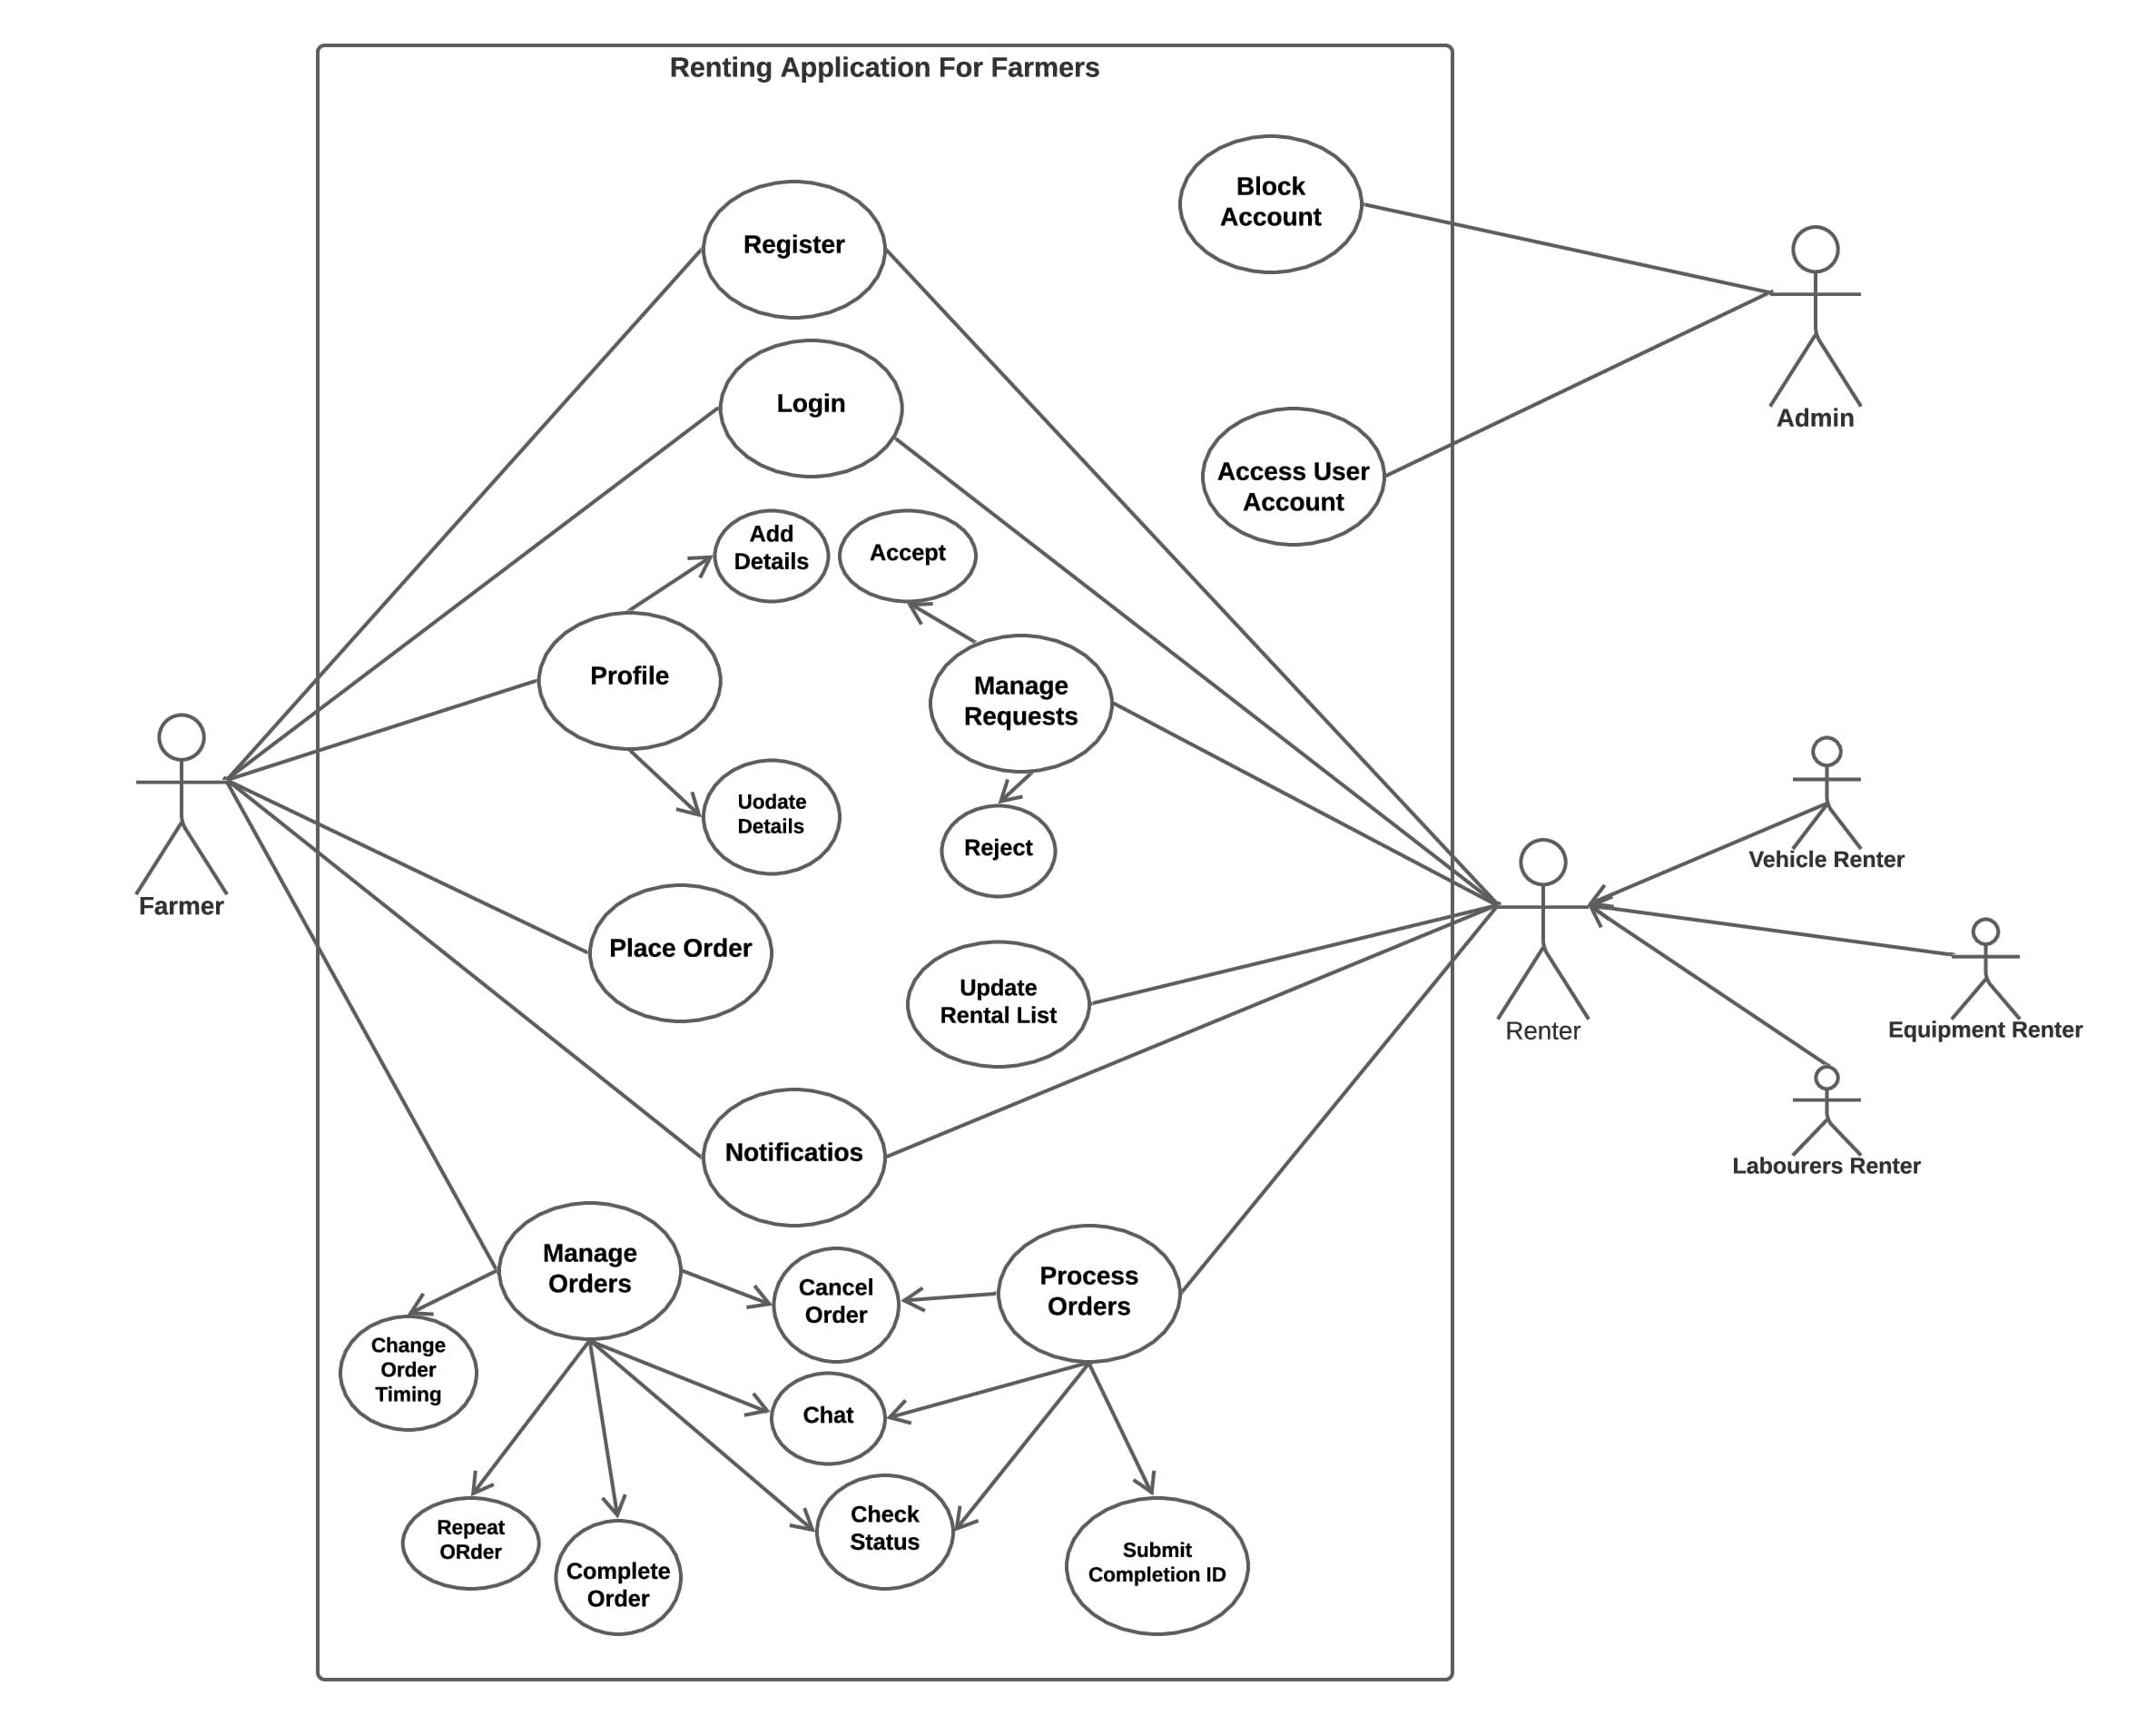
\includegraphics[width=9cm,height=9cm]{UCD}
\caption{Use case}
\label{fig:UCD}
\end{figure}


\section{Implementation details}
\subsection{Front-end}
• Sign in and sign up for views. Interactive functionalities for Sign in and Sign up\\
• create a fire-base to store the received data from the back-end\\
• Ui designing of every page\\
• Add/update vehicles \\
• Process orders\\
• location setting\\ 
• date setting \\
• time setting\\
• User will be notified via gmail\\
• Generating order id for both type's of users\\
• Admin can add users \\
• Admin can update details of users\\

\subsection{Back-end}
• Make a server that is always available to handle each request for the application\\
• Sign in and sign up functions to approve the coming authentication requests from the application\\
• Functions that return required data like order lists, vehicle lists, filter the list of renters according to queries, pass on the updates of orders received from farmer\\
• Maintain the profile of all users according to the schema.\\

\subsection{Connection}
• Define HTTP requests on the Application side to interact with the server and ask for some data or authorise something\\
• make real-time stream through the socket for real-time communication\\



\section{Environment setup}
Installing dependencies\\
1)installing Node via Chocolatey\\
2)open Administrator command prompt run\\ 
"choco install -y nodejs.install openjdk8"\\
3)Download and Install Android Studio\\
4)check following boxes "Android SDK" ,"Android \\
SDK Platform","Android Virtual Device"\\
5)Install Android SDK\\
6)Configure the ANDROID HOME environment variable\\
7)Add platform tools to Path\\
8)Now run "npx react-native init AwesomeProject" \\
to create new project\\
9)compilation and running details has been \\
added below\\

\section{App Compilation and Running}
For compiling and running there are two options\\
1) In real device\\
2) In Android AVD MANAGER\\

I have used "real Device"\\

\subsection{In Real Device}
1)Install Android Studio\\
2)Download SDK managers tools\\
3)Install USB debugging App \\
4)Connect your mobile to computer through USB\\
5)Go to "Open Developer Options"\\
6)Select Developer Option and USB debugging\\
7)Run a Command adb devices\\
8)it will show your devices there \\
9)Now Run a command "npx react-native run-android"\\
10)it will start building  app\\
11)It will download and install App in connected device\\
12)it will compile your code and show App\\
13)to compile your code --> make changes\\
in code and reload it will show output\\

\subsection{In Android AVD MANAGER}
1)Install Android Studio\\
2)Download SDK managers tools in android studio\\
3)Download AVD in indroid studio\\
4)Now open project directory in terminal and run \\
"npx react-native start"\\
5)Metro Bundler will run that terminal through your\\
app compilations \\
6)Now open another project directory in terminal and \\
run "npx react-native run-android"\\
7)It will start building app\\
9)to compile your code --> make changes in code and \\
reload it will show output\\


\section{Manual testing}
\subsection{Use case 1: User Login}
Testing for email verification\\
Test case 1:\\
Custom I/P : dakevan2000@gmail.com\\
Expected O/P : true\\
Actual O/P : true\\
Remark : working fine\\
Test case 2 :\\
Custom I/P : abcd@gmail.com\\
Expected O/P : not registered yet\\
Actual O/P : not registered yet\\
Remark : working fine\\
Test case 3 :\\
Custom I/P : abcd@\\
Expected O/P : invalid email\\
Actual O/P : invalid email\\
Remark : working fine\\
\\

\subsection{Use Case 2: User Signup}
Testing for Email verification:\\
Test case 1 :\\
Custom I/P : 201701182@daiict.ac.in\\
Expected O/P : true\\
Actual O/P : true\\
Remark : working fine\\
Test case 2 :\\
Custom I/P : av.@gmail.com\\
Expected O/P : false\\
Actual O/P : false\\
Remark : working fine\\
Test Case 3 :\\
Custom I/P : acd@gmail\\
Expected O/P : false\\
Actual O/P : false\\
Remark : working fine\\
Test Case 4 :\\
Custom I/P : dakevan2000@gmail.com\\
Expected O/P : Already registered\\
Actual O /P Already registered\\
Remark : working fine\\
Remark : working fine\\



\subsection{Password and confirmed password should be matched}
Test Case 1:\\
Custom I/P : (1) abcdef (2) abcdef\\
Expected O/P : true\\
Actual O/P : true\\
Remark : working fine\\
Test Case 2:\\
Custom I/P : (1) abcdef (2) abcdea\\
Expected O/P : false\\
Actual O/P : false\\
Remark : working fine\\

\subsection{ mobile number}
Test Case 1:\\
Custom I/P : 1234567890\\
Expected O/P : true\\
Actual O/P : true\\
Remark : working fine\\
Test Case 2 :\\
Custom I/P : 123456\\
Expected O/P : false\\
Actual O/P : false\\
Remark : working fine\\
Test Case 3:\\
Custom I/P : 12345678901\\
Expected O/P : false\\
Actual O/P : false\\
Remark : working fine\\

\section{system testing}
1) Negative testing : \\
--While sign up I entered the wrong name and the wrong \\
email format to test it allow me to sign up  or not \\
--While changing the password i entered the wrong \\
password to see it password or not\\
--While ordering Vehicle/equipment I didn't enter mandatory \\
filled to test an order will be placed or not\\
--while ordering Vehicle/Equipment i enter wrong email\\
format to test it place order or not\\
Like this i test functionalities of application.\\
\\
2) Usability testing\\
I run this application in front of users of this application\\
and non users of this application to test what users feel about\\
this application\\
-- I run my app in front of farmers to test what they feel about\\
application\\
-- I run my app in front of engineers(my college friends) \\
to test what they feel about application\\
\\
Functional testing : I have taken lot of farmers interview \\
to know about what types of functionalities they want?\\
-- Farmers can order every vehicle and equipment\\ 
-- Farmers can place multiple orders\\
Non Functional testing : As i was developer of this i thought\\
-- Farmers can repeat same order by changing date and time\\
-- Farmers can Delete their account\\
-- Farmers can update their details
-- Farmers will get mail confirmation after placing orders\\


\section{acknowledgement}
I would like to thank professor JayPrakash Lalchandani for his guidance throughout the BTP. He guides me very well. He is such a good mentor to me, because of that I have completed this application without any experience. I also want to thank BTP coordinator prof. Gagan Gard for his support throughout the BTP completion.\\

\section{References}
• Introduction to React Native Document\\
• Toward Better Documentation : React-Native\\
• react-native-document-picker\\
• Yarn packages manager\\
• React js: A JavaScript library for building user\\
interfaces\\
• Geeksforgeeks\\

\begin{figure}[h!]
\centering
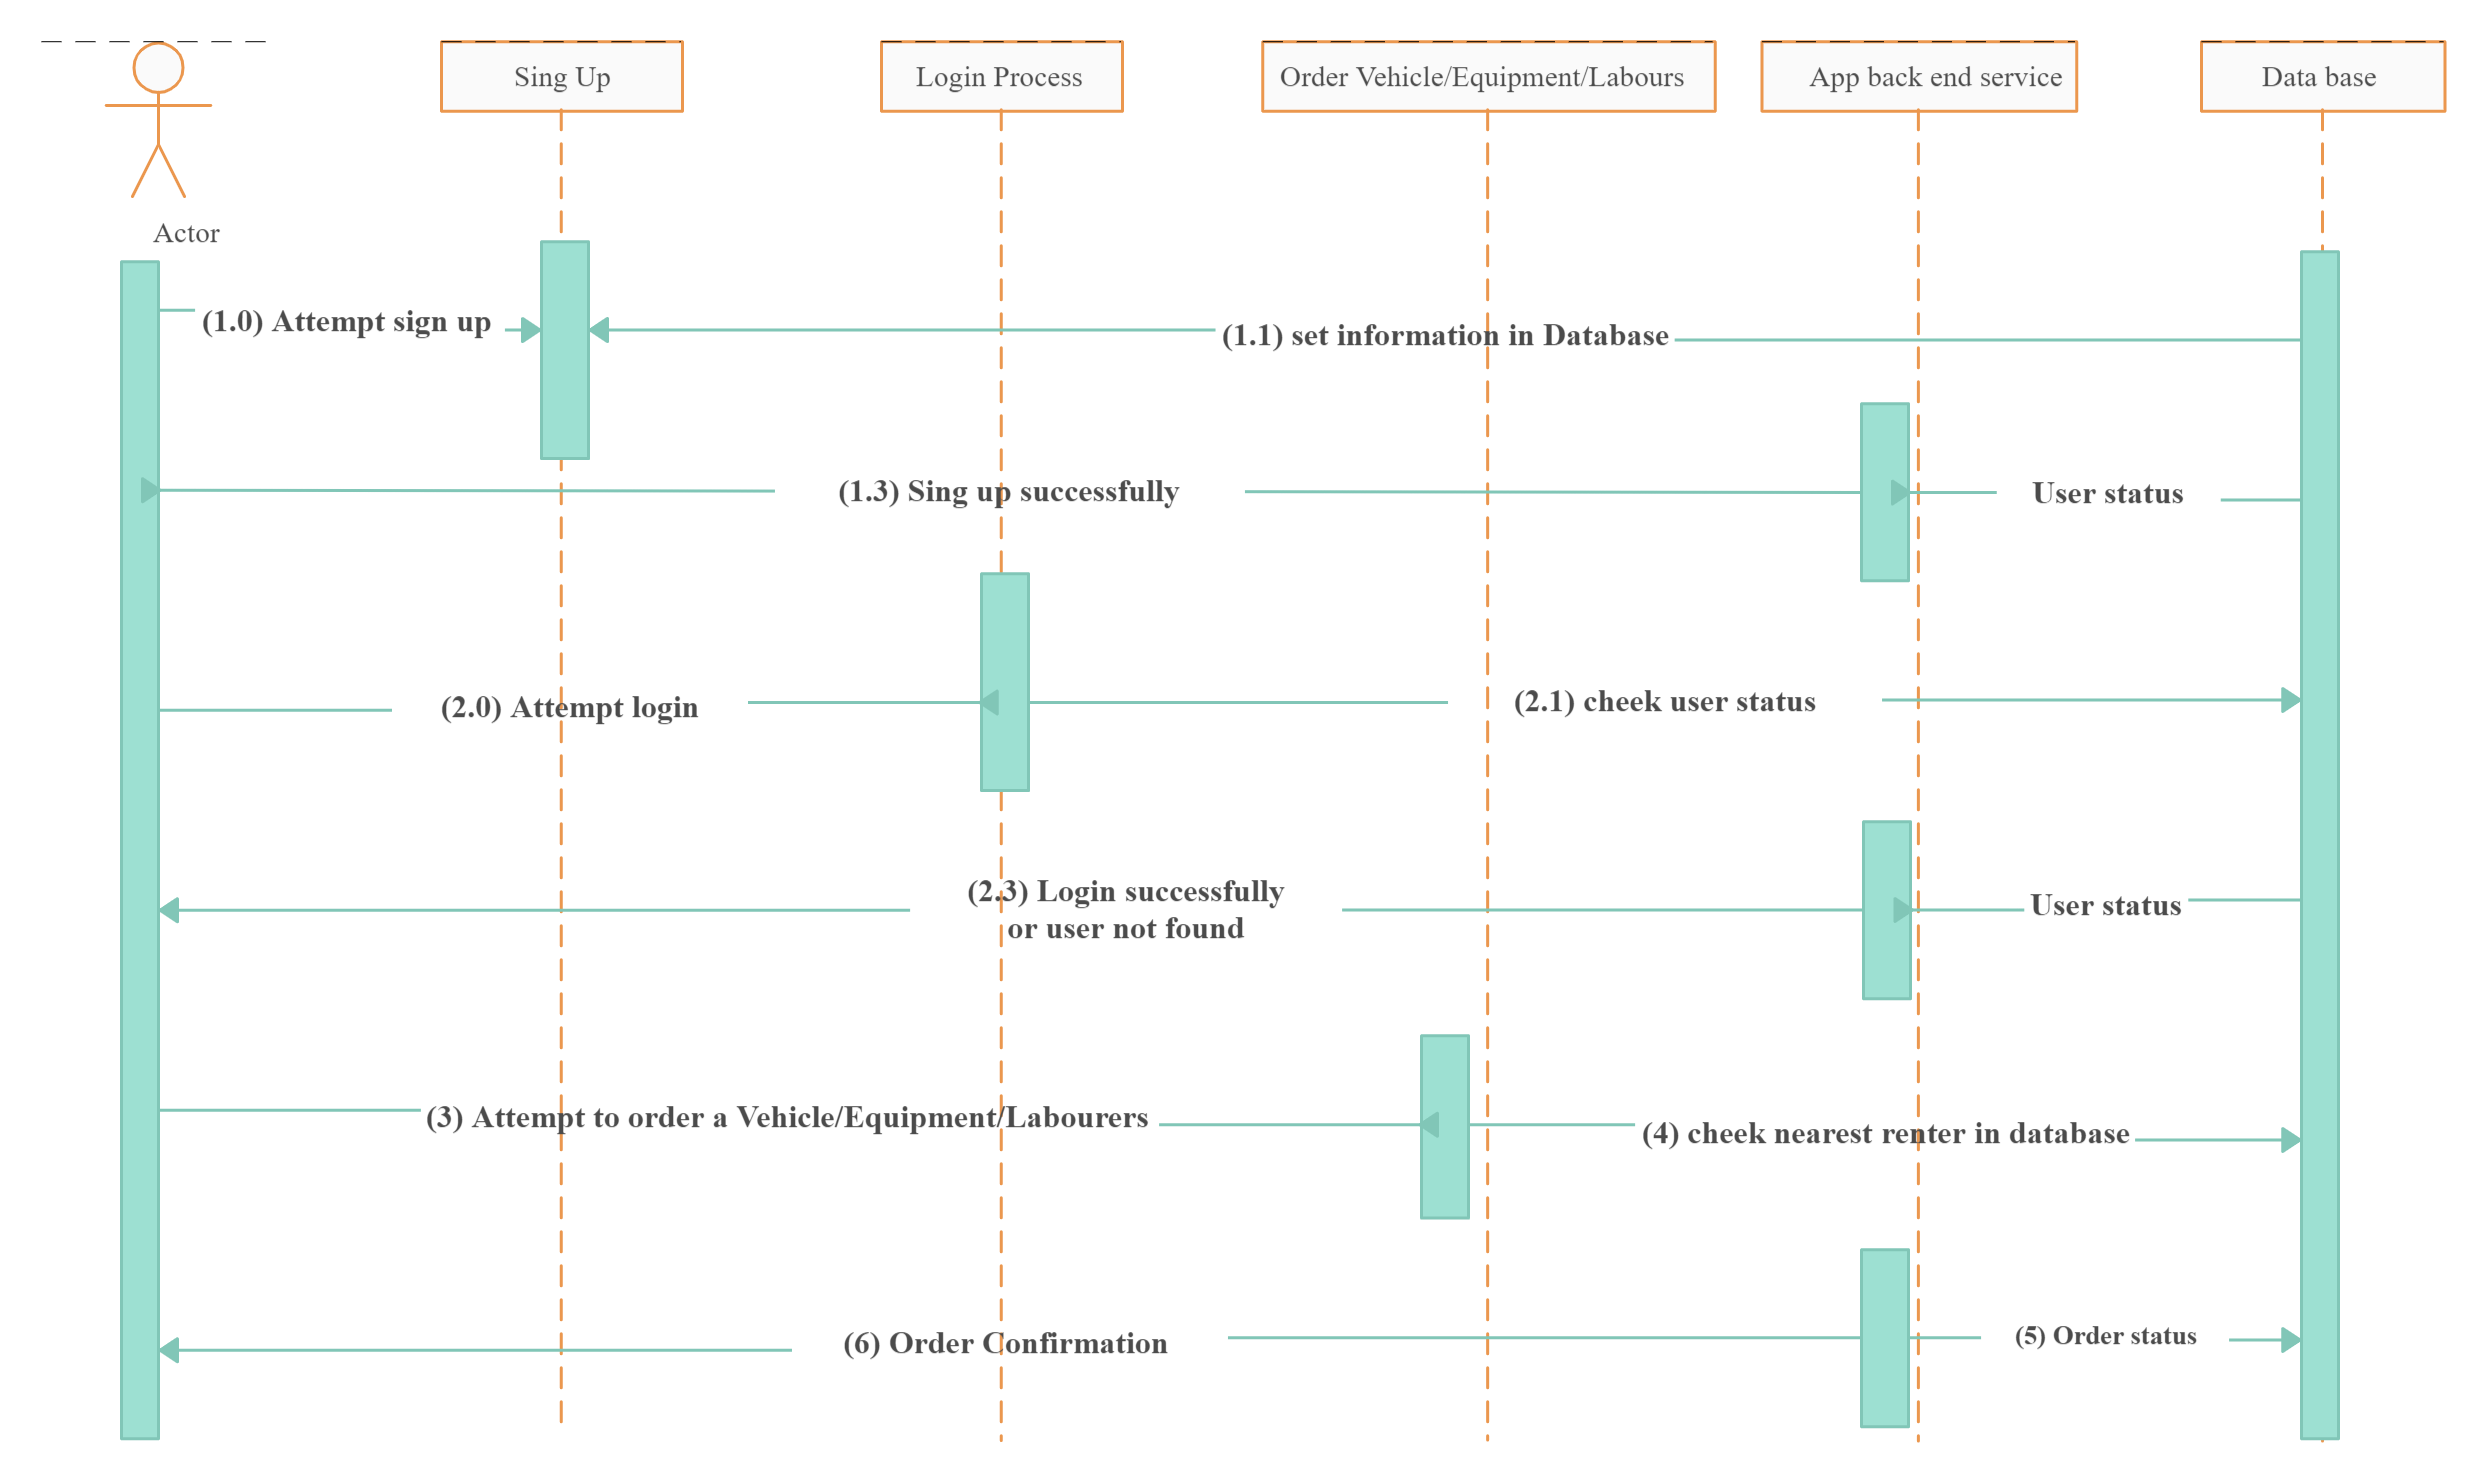
\includegraphics[width=11cm,height=13cm]{UMLS}
\caption{UML Sequence Diagram}
\end{figure}


\begin{figure}[h!]
\centering
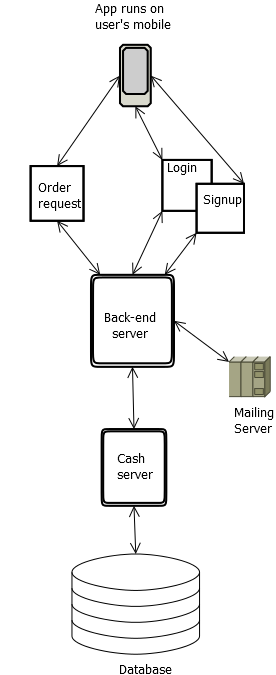
\includegraphics[width=5cm,height=13cm]{images/Architecture.png}
\caption{System Architecture Diagram}
\end{figure}




\begin{figure}[h!]
\centering
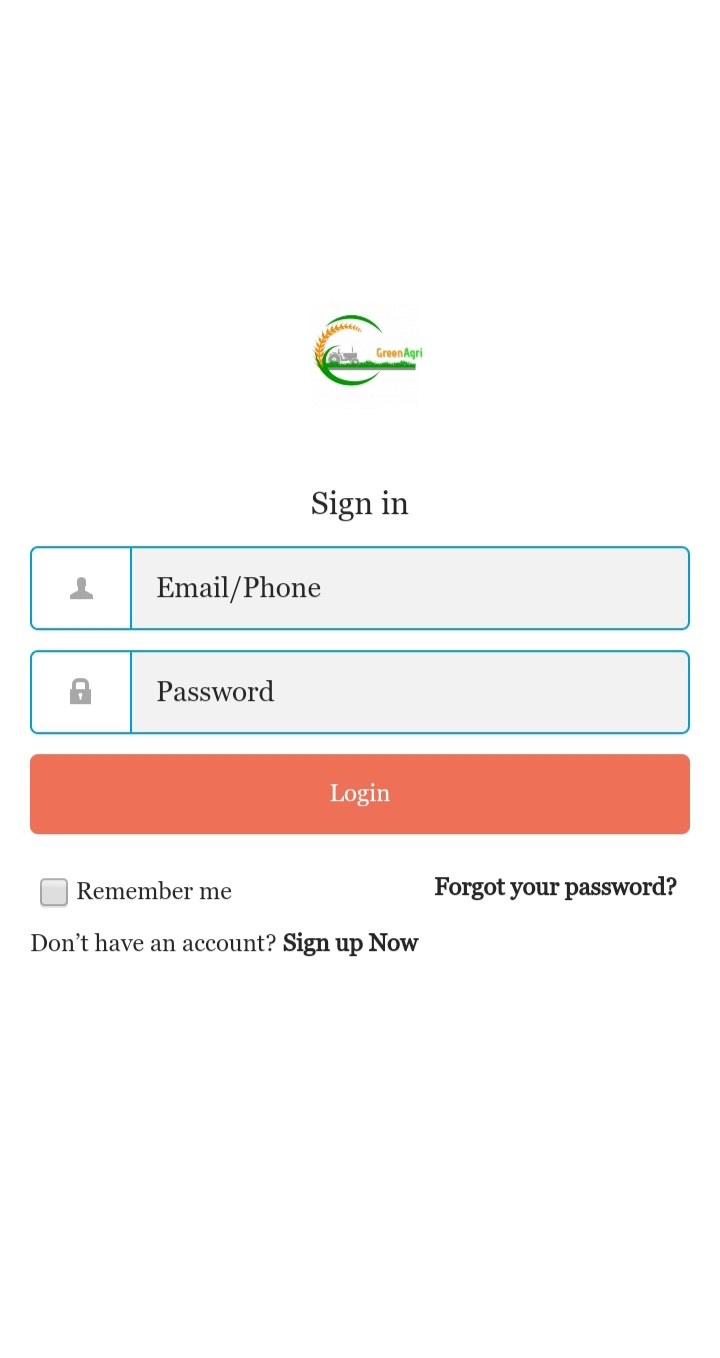
\includegraphics[width=5cm,height=9cm]{Signin}
\caption{Signin page}
\label{fig:Signin}
\end{figure}



\begin{figure}[h!]
\centering
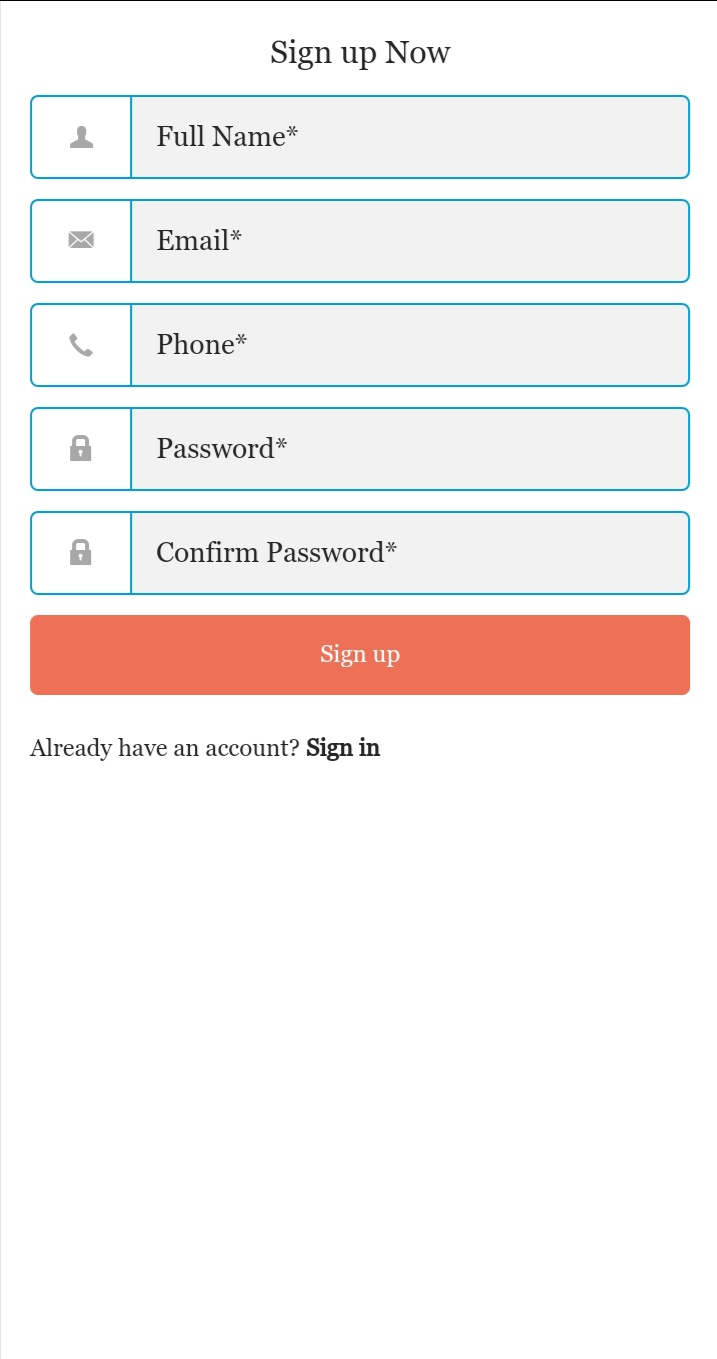
\includegraphics[width=5cm,height=9cm]{Signup}
\caption{Signup page}
\label{fig:Signup}
\end{figure}


\begin{figure}[h!]
\centering
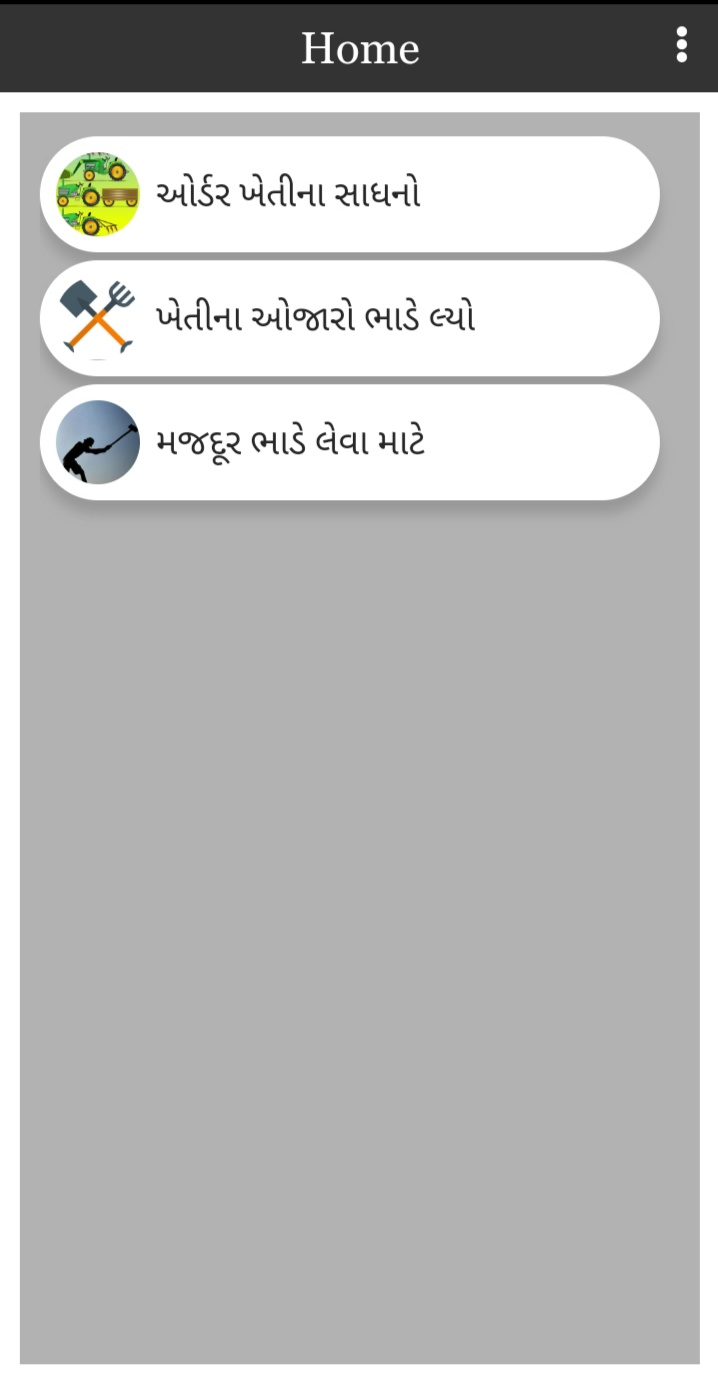
\includegraphics[width=5cm,height=9cm]{Home}
\caption{Home page}
\label{fig:Home}
\end{figure}

\begin{figure}[h!]
\centering
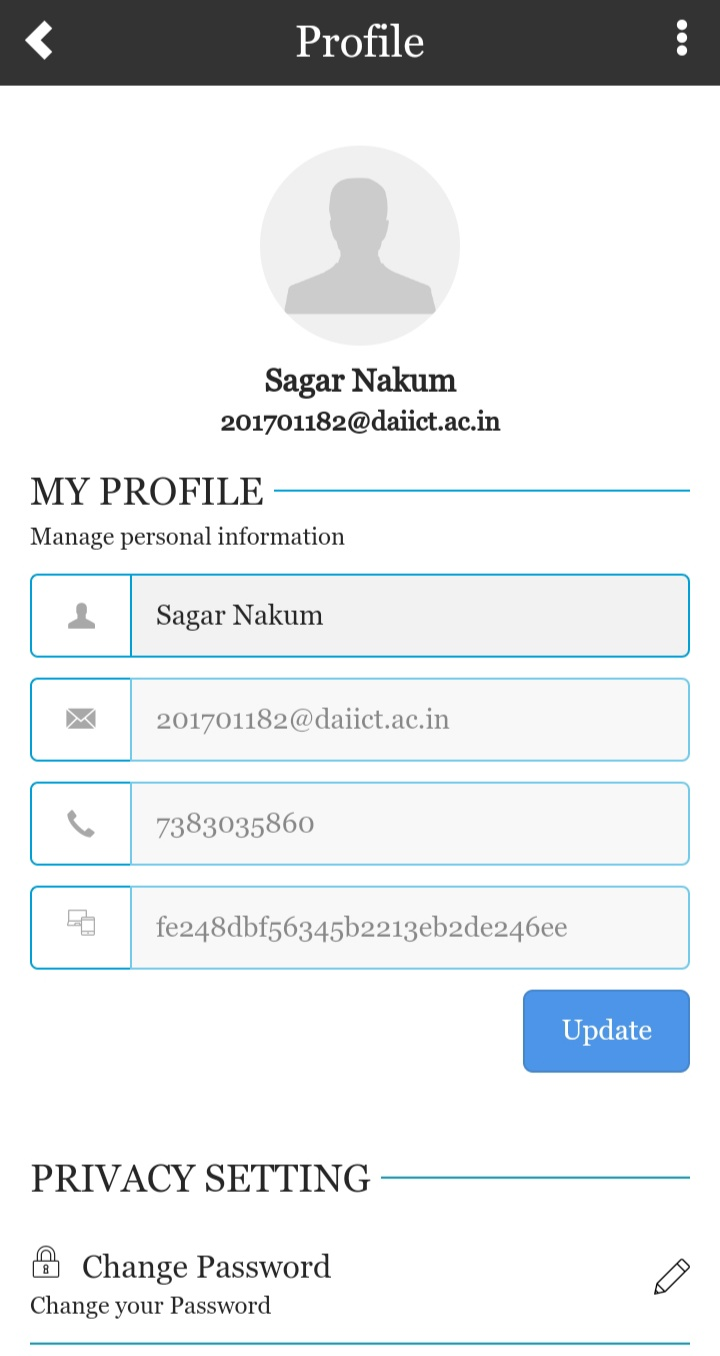
\includegraphics[width=5cm,height=9cm]{Profile1}
\caption{Profile}
\label{fig:Profile1}
\end{figure}


\begin{figure}[h!]
\centering
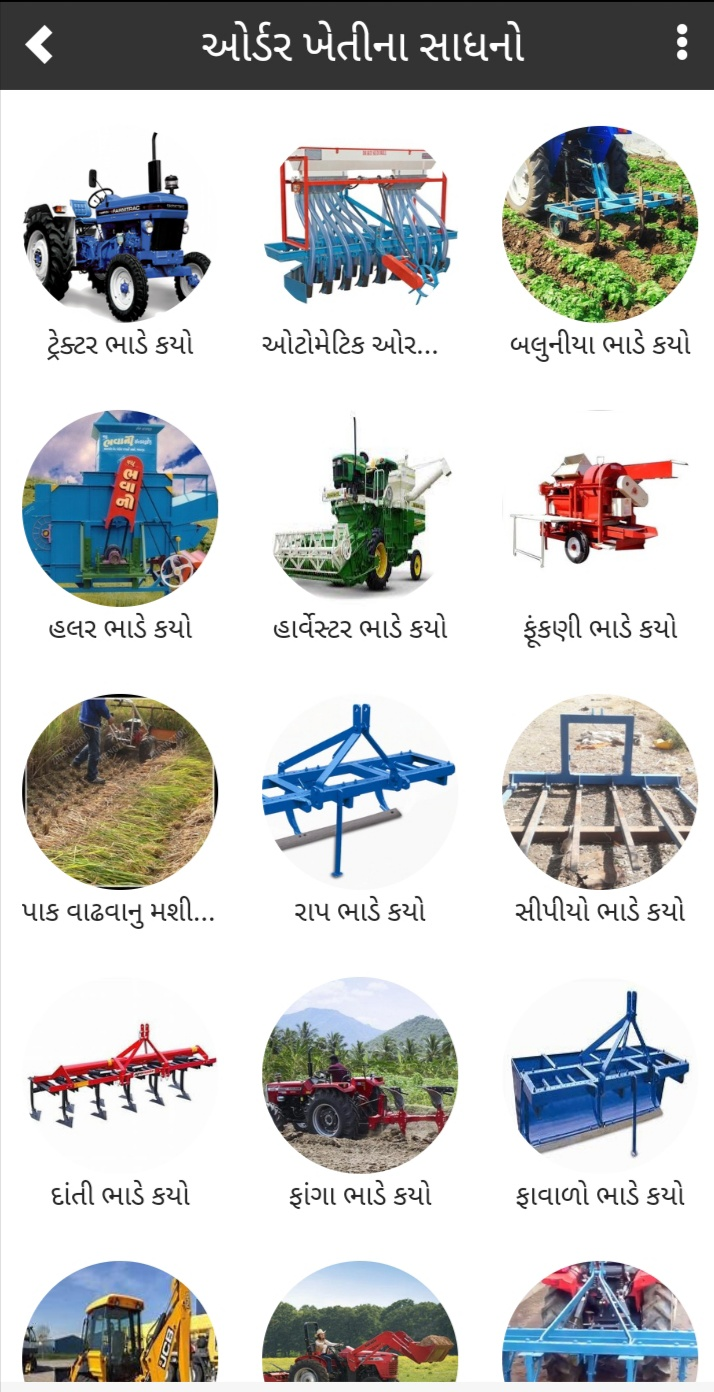
\includegraphics[width=5cm,height=9cm]{Vehicle1}
\caption{Order Vehicle}
\label{fig:Vehicle1}
\end{figure}

\begin{figure}[h!]
\centering
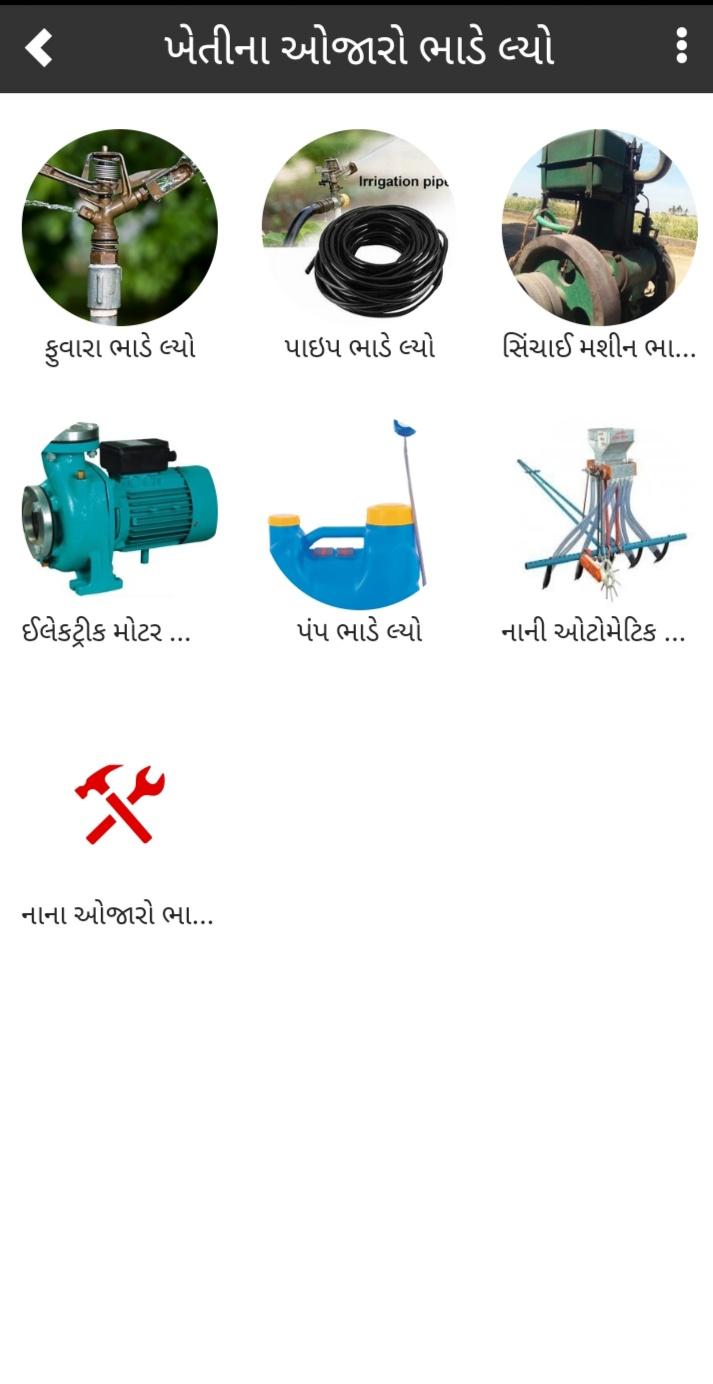
\includegraphics[width=5cm,height=9cm]{Equipment}
\caption{Order equipment}
\label{fig:Equipment}
\end{figure}

\begin{figure}[h!]
\centering
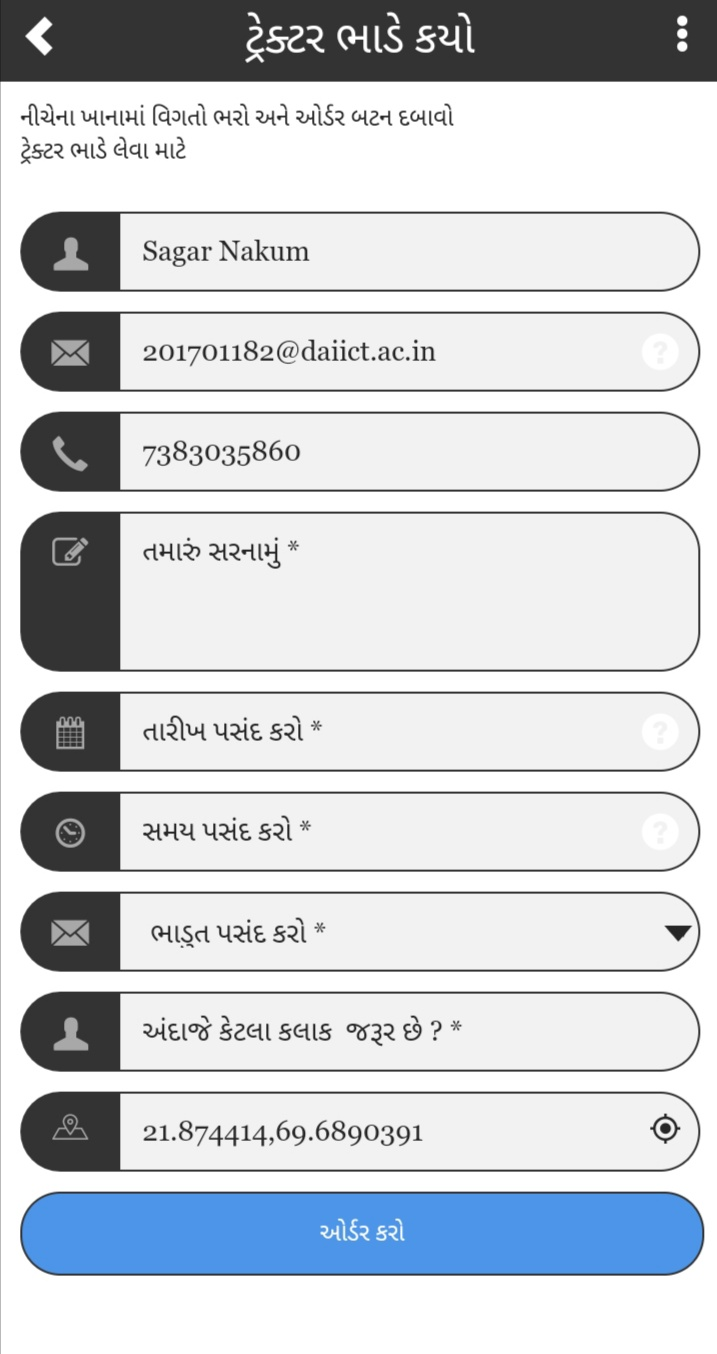
\includegraphics[width=5cm,height=6cm]{Tractor}
\caption{Vehicle Order page}
\label{fig:Tractor}
\end{figure}

\begin{figure}[h!]
\centering
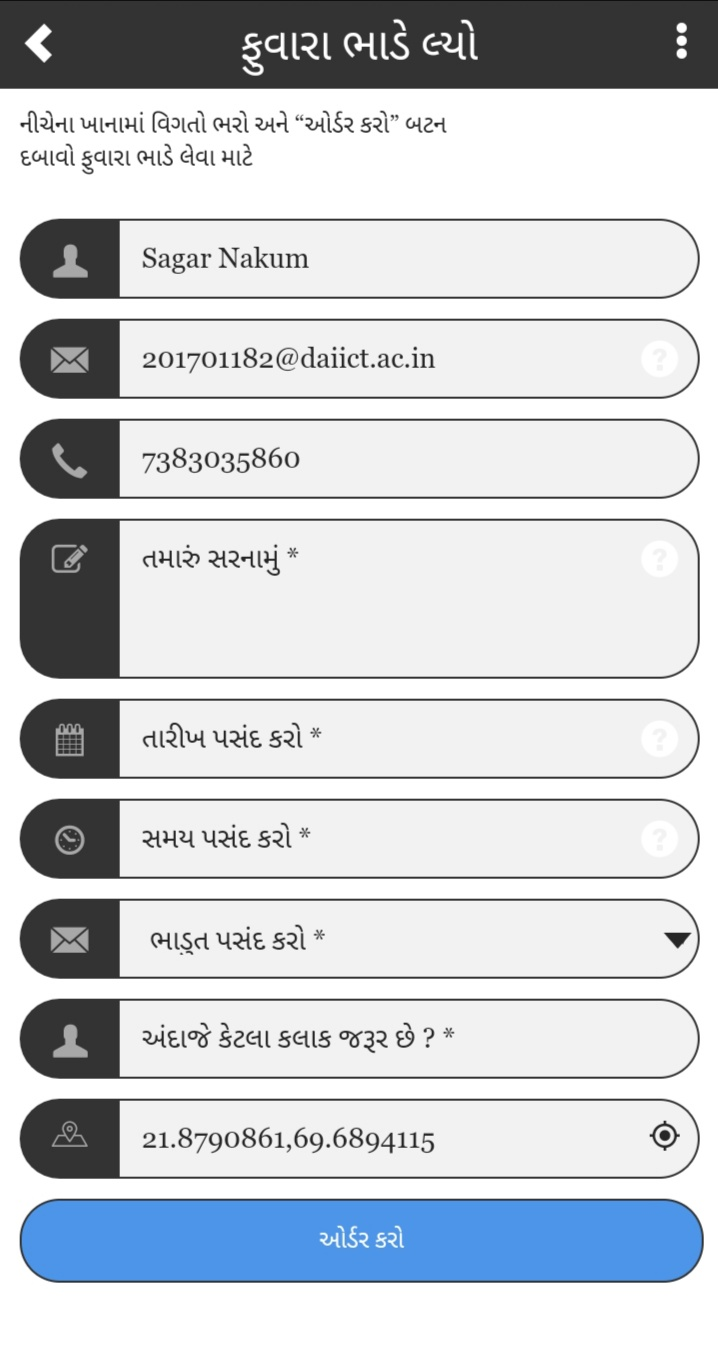
\includegraphics[width=5cm,height=6cm]{Fuva}
\caption{Equipment Order page}
\label{fig:Fuva}
\end{figure}

\begin{figure}[h!]
\centering
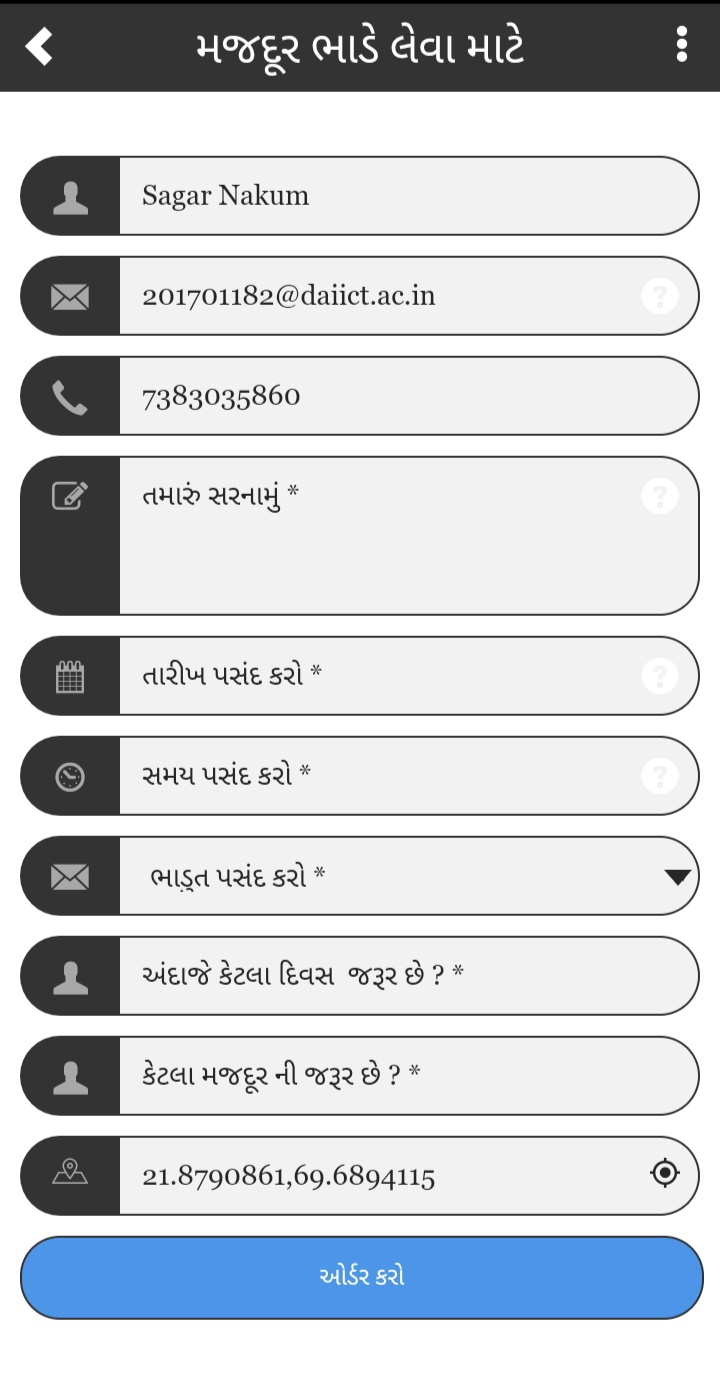
\includegraphics[width=5cm,height=6cm]{Labours}
\caption{Labours Order page}
\label{fig:Labours}
\end{figure}
\newpage





\begin{figure}[h!]
\centering
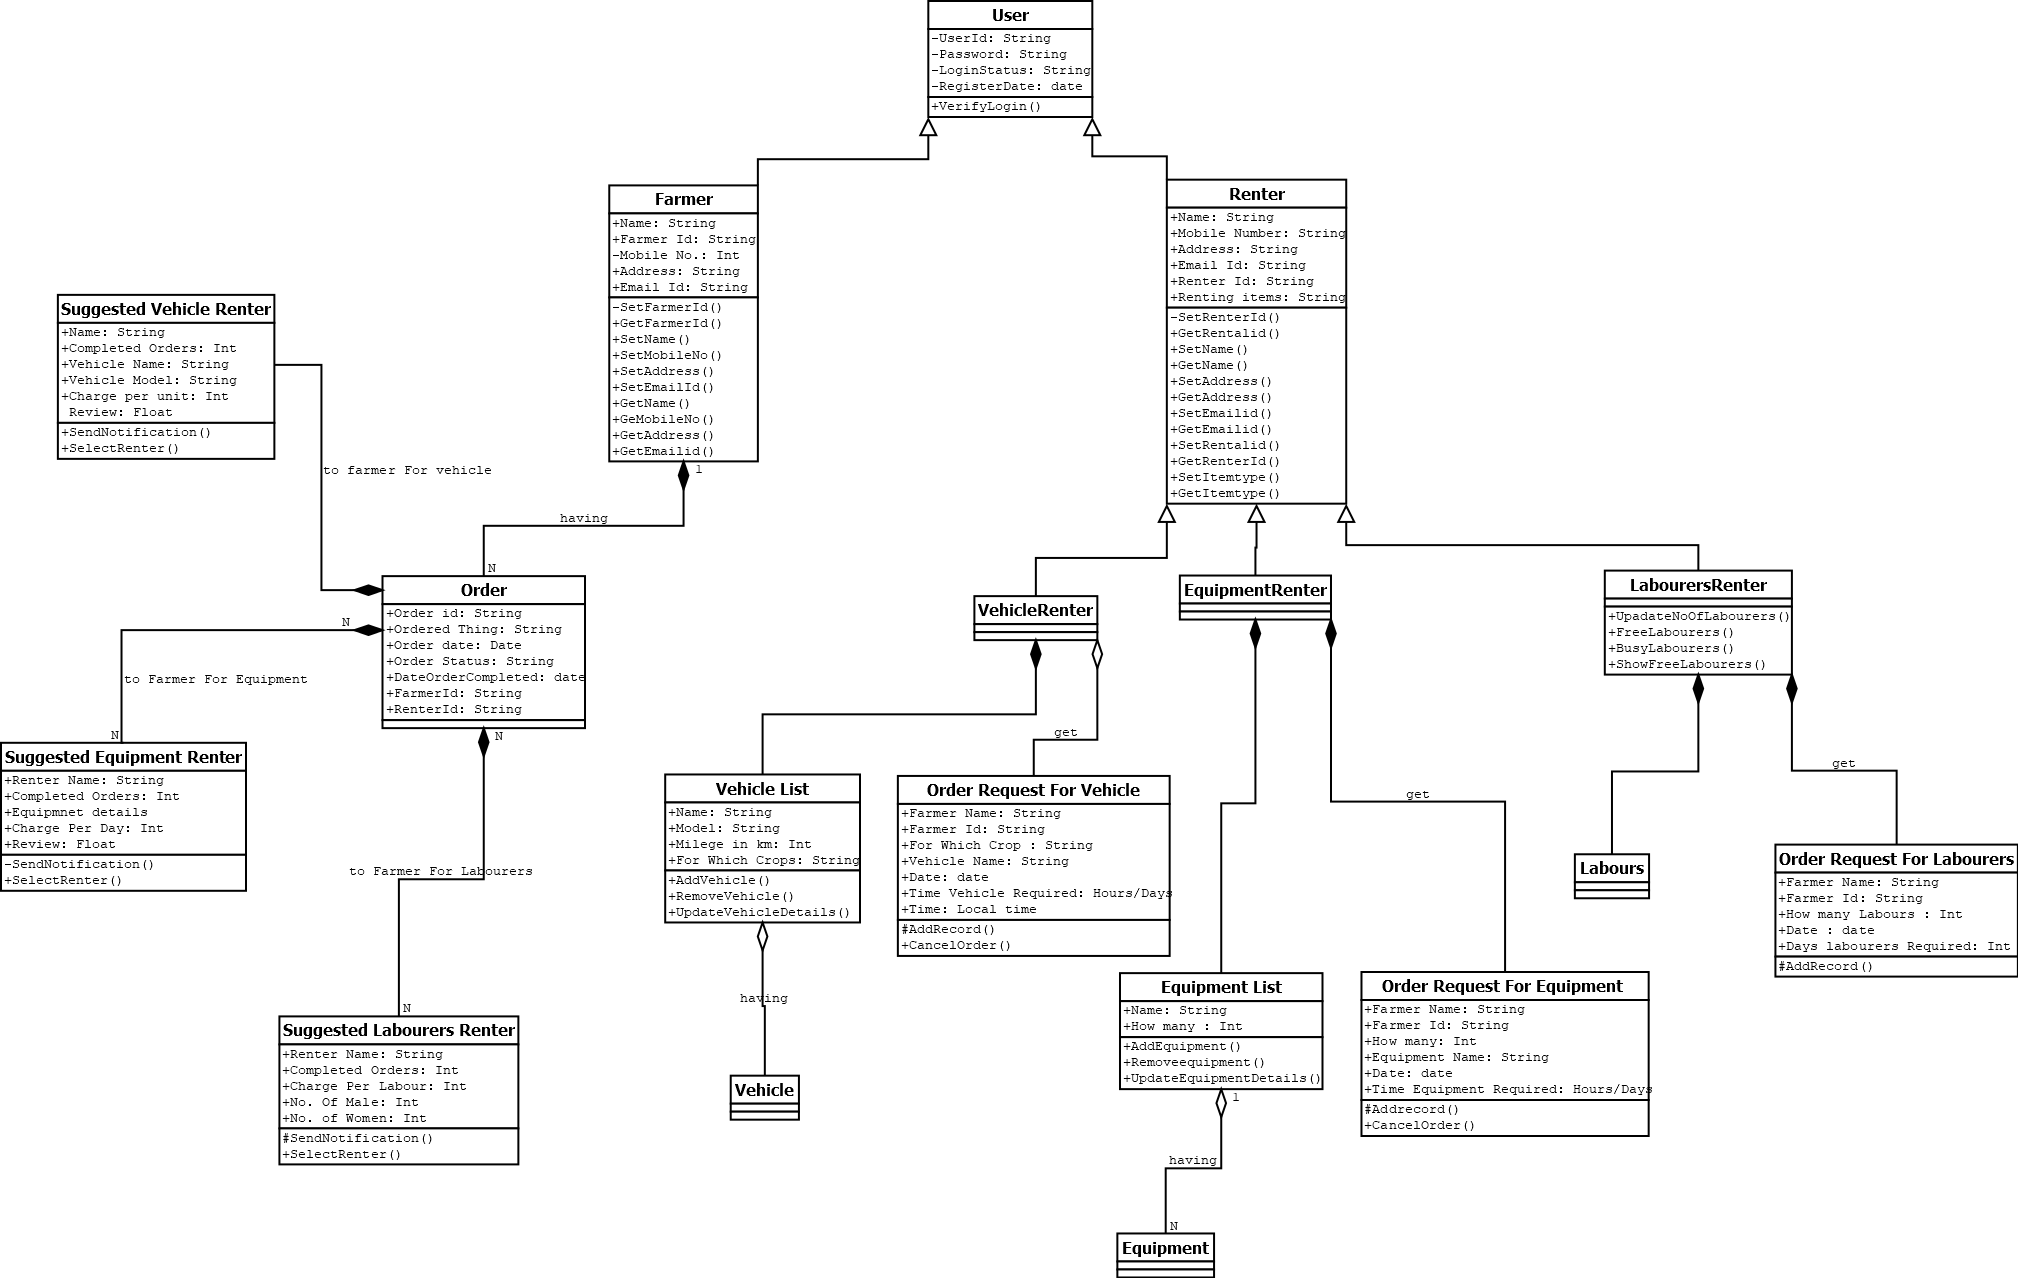
\includegraphics[width=19.5cm,height=20cm]{UML}
\caption{UML Class diagram}
\label{fig:UML}
\end{figure}


\end{document}
